\chapter{Hra PolyBridge}

Poly Bridge je logická simulovaná hra, která byla vyvinuta nezávislým vývojářským týmem Dry Cactus. Hráči mají za úkol navrhovat mosty, které musí odolat zátěži projíždějících vozidel a zároveň splňovat omezení daná rozpočtem a dostupnými materiály. Díky svému základu v realistické fyzice nabízí Poly Bridge možnost experimentovat s různými stavebními technikami a materiály.

Zajímavým aspektem hry je také komunitní prvek. Hráči mohou sdílet své vlastní návrhy mostů a úrovní online, kde je mohou ostatní hráči testovat a hodnoti. Díky tomu, je možné sdílet techniky a nápady mezi hráči z celého světa. 

"Popusťte uzdu své inženýrské kreativitě v poutavém a neotřelém simulátoru stavby mostů se všemi zvonky a píšťalkami. Užijte si hodiny řešení fyzikálních hádanek v kampani a pak se vrhněte do sandboxu a vytvářejte vlastní návrhy mostů a hádanky!" (přeloženo Dry Cactus citace)

\section{Vlastní hra}

Samotná hra se skládá ze 7 kampaní. V každé kampaní se nachazí 15 různých úrovní, které se postupně zvyšují v obtížnosti.

Po výběru úrovně je hráči představeno prostředí, které se ve většině případů skládají z levého a pravého břehu, řeky a jednoho nebo více vozidel. K dispozici je řada materiálů, jako je dřevo, vozovka, ocel, hydraulika a další. Materiály se od sebe liší svou nosností, maximální délkou a cenou.

Hráč nejdříve vytvoří svůj návrh a realizuje ho klikáním na předem určené body v prostředí. Kliknutím na dva body se mezi nimi vytvoří vybraný materiál. Pokud se dva materiály potkají na stejném bodě, vytvoří se mezi nimy volně pohyblivý kloub. V prostředí jsou předem některé body vybrané jako kotvy. Tyto kotvy jsou nepohyblivé a hráč na ně může navázat stavou svého mostu a získat tím oporu pro jeho výtvor.

Když je hráč se svým návrhem a realizací spokojený, může spusti simulaci. Během simulace není možné přídávat další materiály. Vozidla začnou jezdit z jedné strany mostu na druhou a hráč sleduje, zda konstrukce vydrží. Pokud most selže, hráč musí identifikovat slabá místa a provést potřebné úpravy.

Proces návrhu, testování a úprav se opakuje, dokud most nevydrží požadované zatížení bez překročení rozpočtu.

\xxx{Můžu sem dát odkaz např. na trialer na hru z youtube? Nebo možná screenshoty ze hry?}

\begin{figure}[p]\centering
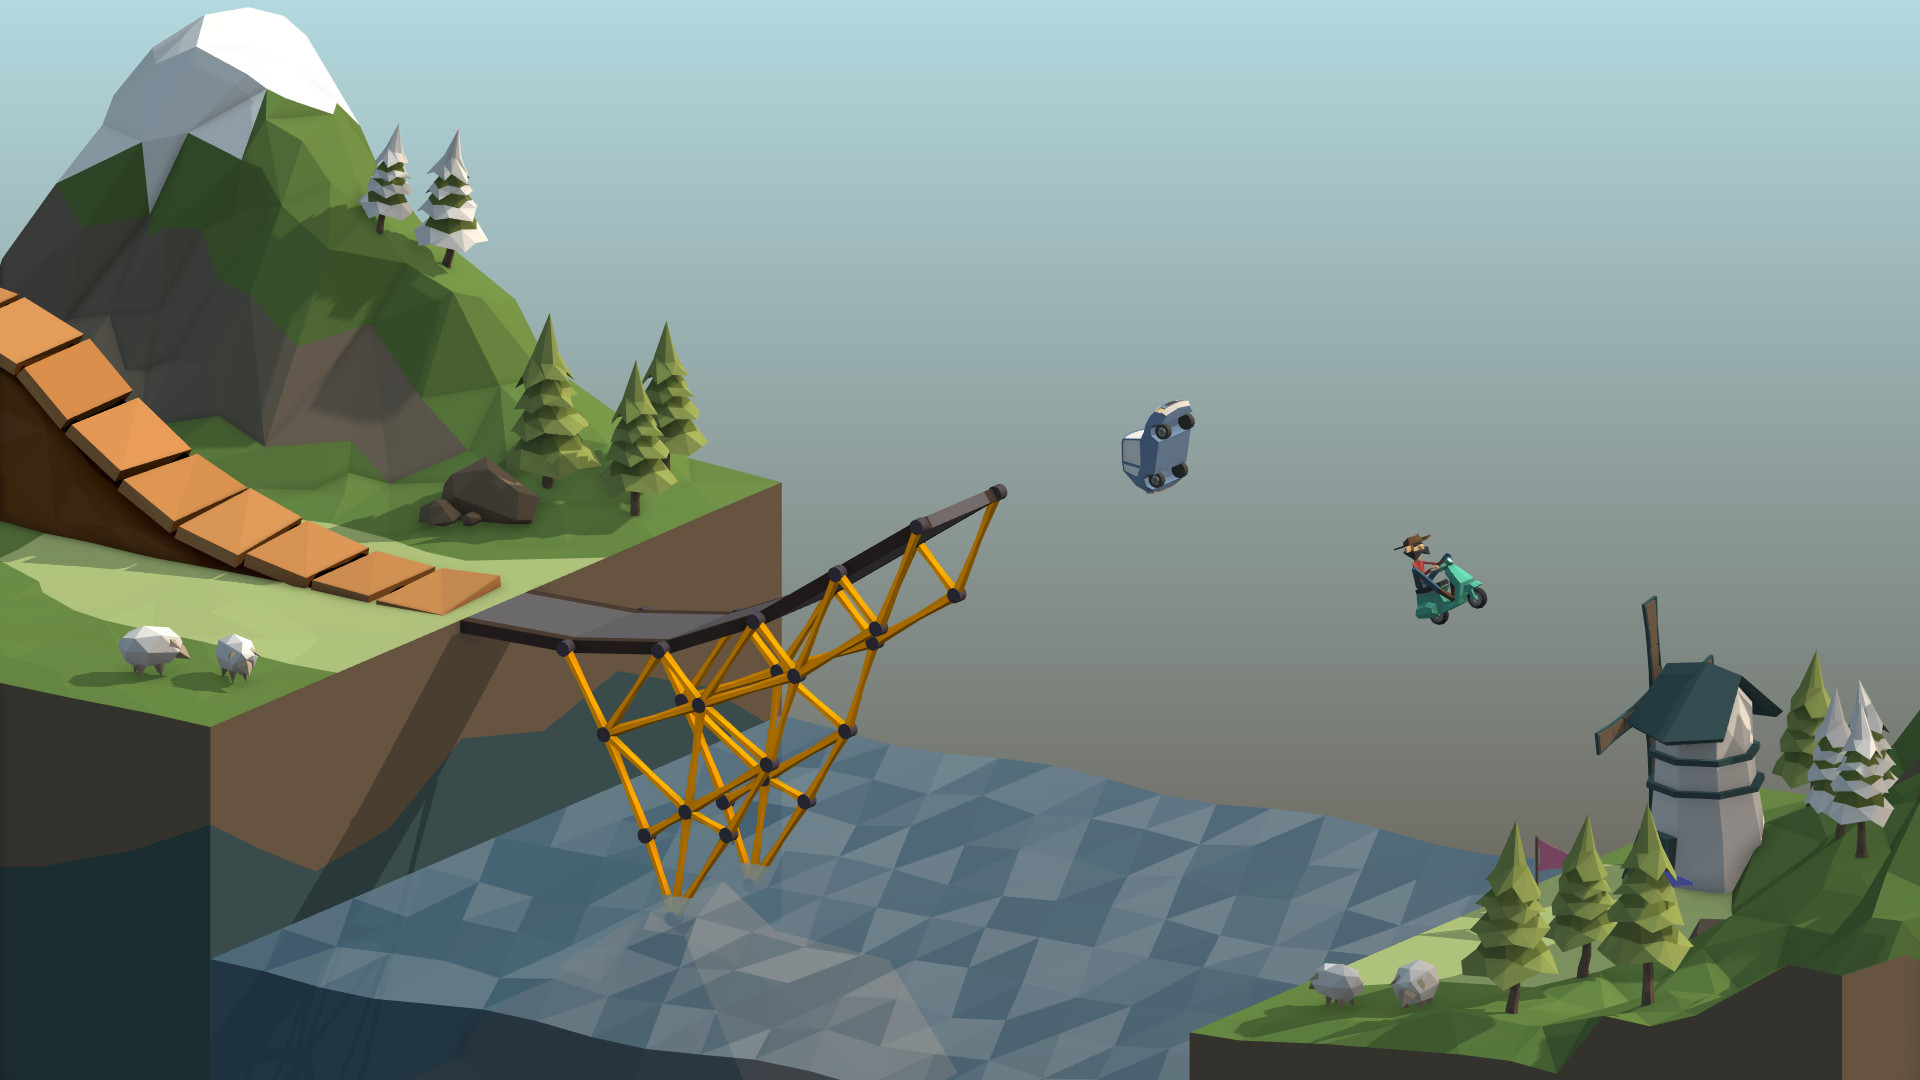
\includegraphics[width=140mm, height=140mm]{img/poly_screen_1.jpg}
\caption{Ukázka ze hry polybridge}
\label{fig:5}

\end{figure}

\begin{figure}[p]\centering
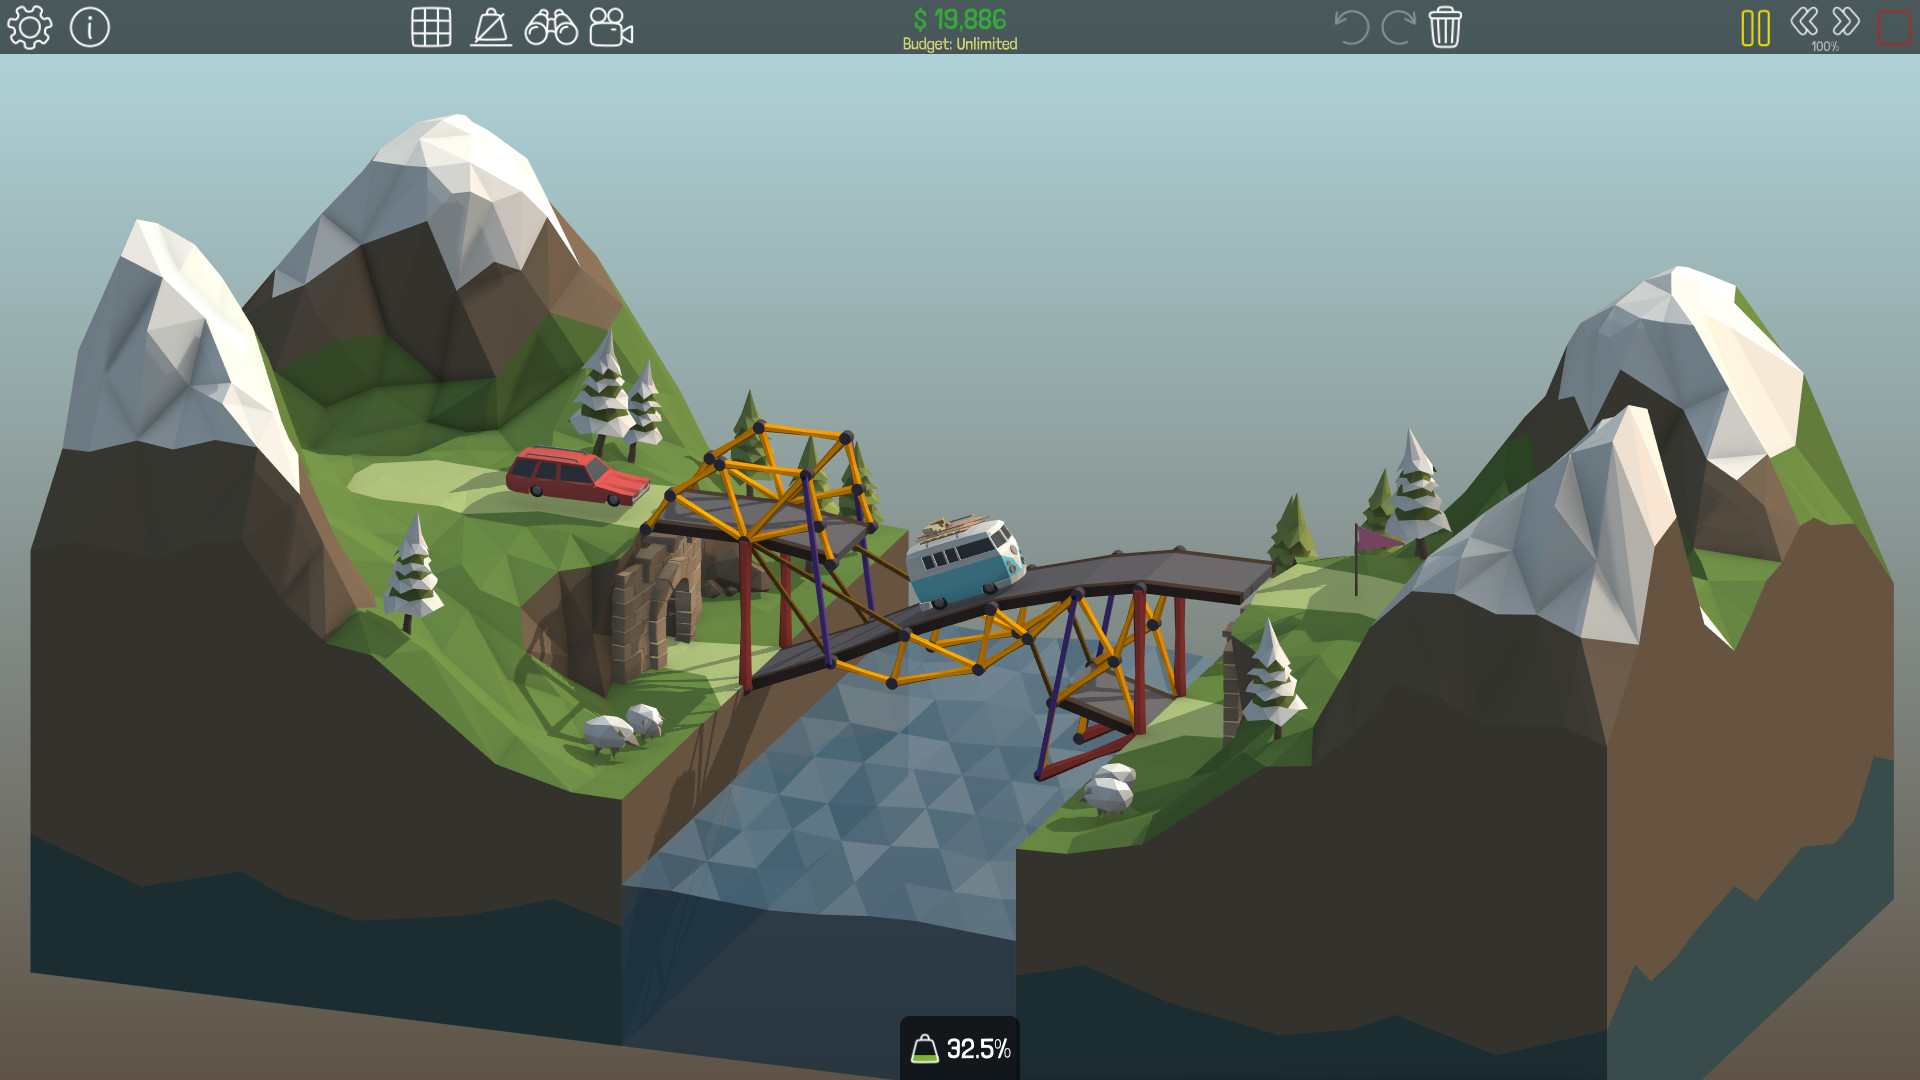
\includegraphics[width=140mm, height=140mm]{img/poly_screen_2.jpg}
\caption{Ukázka ze hry polybridge}
\label{fig:6}
\end{figure}



